\chapter{LapOps}
The following chapters will deal with the idea, concept, implementation and application of an Android App developed within the Embedded Systems workshop called LapOps.
\begin{figure}[H]
	\centering
	
\includegraphics[scale= 0.5]{Pictures/lapops-icon.png}
	\caption{LapOps icon}
	\label{icon}
\end{figure}


\section{Introduction}
The sections below will give a brief introduction of the project's team and the idea. The second chapter will cover the system analysis which contains use cases and a small state machine. The following chapter consists of the gathering, modification and analysis of data to achieve the goals set for the application. This chapter will also cover the mathematical fundamentals needed to work with the collected data. Following this, the application usage is explained in chapter \ref{manual}. The last chapter gives the conclusion to the project.

\section{Team}
The team consists of two Computer Scientists and one Mathematician. All of us are working for IT-Designers GmbH in Esslingen. The Project Lead is taken by Stephan Dittmann. Further roles are split between every project team member.

\section{Core Idea of the Project}
The idea behind the project was to create an application that records a driven lap with a car or a go-kart and returns a result, that identifies the fastest lap and compares other laps to it. Our core problem, that we identified in our project is the identification of the track sections. After discussion, we reached a consensus, that our application should be able to identify curves and straights reliable. The first sketch is visible in figure \ref{sketchLapOps} which shows the idea of splitting a track into sections. The last step would be to compare the same sections in different laps to get improvement tips.

\begin{figure}[H]
	\centering
	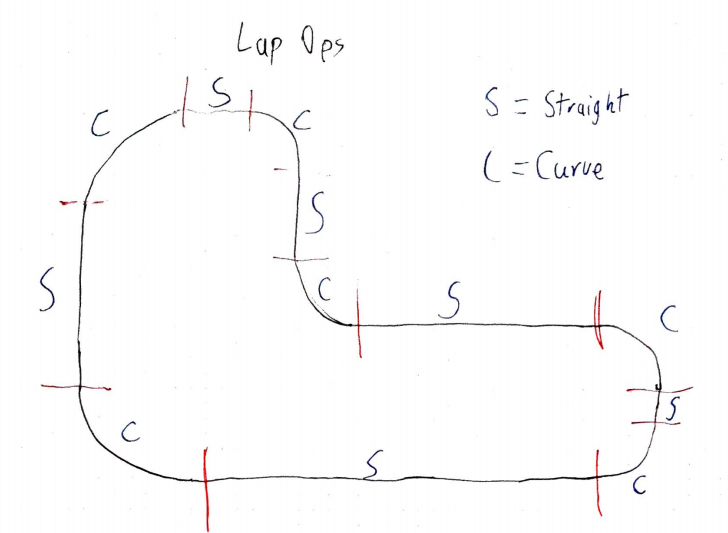
\includegraphics[scale= 0.6]{Pictures/LapOpsSkizze.png}
	\caption{Sketch of the core idea of section identification}
	\label{sketchLapOps}
\end{figure}
